\documentclass{cmn}
\usepackage{pgfplots}
\pgfplotsset{compat=1.18}
\usepgfplotslibrary{units}

\begin{document}
  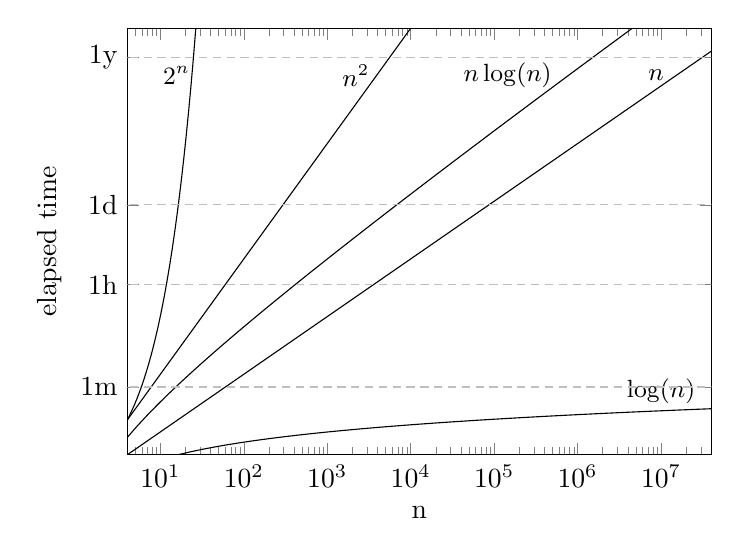
\begin{tikzpicture}
    \begin{loglogaxis}[
      width=90mm,
      height=70mm,
      xlabel={n},
      ylabel={elapsed time},
      xmin=4,
      xmax=40000000,
      ymin=4,
      ymax=100000000,
      restrict y to domain=1:100000000,
      ytick={\empty},
      extra y ticks={60,3600,86400,31536000},
      extra y tick labels={1m, 1h, 1d, 1y},
    ]
      \addplot [domain=4:100000000,samples=50] { log2(x) } node[above=2mm,left=5mm] {\small $\log (n)$};
      \addplot [domain=4:100000000,samples=30] { x } node[below=6mm,left=9mm] {\small $n$};
      \addplot [domain=4:4525000,samples=50] { x * log2(x) } node[below=6mm,left=9mm] {\small $n \log (n)$};
      \addplot [domain=4:10000,samples=30] { x^2 } node[below=6mm,left=4mm] {\small $n^2$};
      \addplot [domain=4:26.6,samples=30] { 2^x } node[below=6mm,left=-0.5mm] {\small $2^n$};

      \addplot [domain=2:40000000,lightgray,densely dashed] { 60 };
      \addplot [domain=2:40000000,lightgray,densely dashed] { 3600 };
      \addplot [domain=2:40000000,lightgray,densely dashed] { 86400 };
      \addplot [domain=2:40000000,lightgray,densely dashed] { 31536000 };
    \end{loglogaxis}
  \end{tikzpicture}
\end{document}
